\chapter[Nível de Programa]{Nível de Programa}
Nesse nível as atividades executadas foram: Levantar \textit{Features},
Construir Visão, Construir \textit{Roadmap}, Identificar Requisitos Não Funcionais,Escrever
Histórias e Planejar \textit{Release}. 

\section{Requisitos Identificados}

Nesse nível foram identificadas as \textit{features}, que são serviços que o sistema deve fornecer, e os requisitos não funcionais da aplicação.

\subsection{\textit{Features}}
\textbf{\textit{Feature} 01:} FT-01 Listagem de contato de possíveis clientes

Nesta \textit{feature}, espera-se obter uma lista de contatos oriunda de registros, fornecendo portanto a oportunidade de edição e visualização de todos os contatos, assim como seus respectivos atributos e desejos.


\textbf{\textit{Feature} 02:} FT-02 Padronização da divulgação dos serviços

A partir de tal \textit{feature}, há o objetivo de incluir um padrão de apresentações para melhor abordar os clientes. Com isso, um ponto a ser agregado é a forma com que os emails serão enviados além de fornecer a visualização dos serviços que serão oferecidos pela empresa no presente período de tempo.


\textbf{\textit{Feature} 03:} FT-03 Acompanhamento do contato com o cliente

Essa \textit{feature}, é responsável por controlar o oferecimento dos serviços aos clientes através do contatos estabelecidos. Além desse cenário favorável, deve-se registrar os clientes que rejeitaram a proposta em um primeiro momento e anotar seu \textit{feedback}, caso haja.


\textbf{\textit{Feature} 04:} FT-04 Acompanhamento das reuniões com o cliente

Nesta \textit{feature}, espera-se fazer todo o tratamento que envolve as reuniões, desde o seu planejamento, no que se refere as datas e locais, assim como a pauta do que será falado, até uma geração de relatórios do que foi debatido na mesma.		


\textbf{\textit{Feature} 05:} FT-05 Controle das informações referentes ao projeto

Busca-se obter a partir de relatórios, o que de fato está sendo realizado no projeto, se está sendo feita da melhor maneira. Há opções capazes de realizar registros de novos projetos, custos, pessoas envolvidas e avaliar se o projeto é de fato viável.

\subsection{Requisitos Não Funcionais}
Os requisitos não funcionais identificados podem ser vistos na seção 6 do documento de visão que encontra-se no Apêndice \ref{visao}.

Uma vez que as \textit{features} foram identificadas e especificadas, sabe-se que cada uma possui algumas histórias de usuário, que nada mais são do que pequenas descrições que se espera que a aplicação forneça. Abaixo estão listadas as histórias escritas pelos \textit{Product Managers}. Cada história é composta por pessoas em seus devidos papéis que utilizarão a funcionalidade.

\subsection{Papéis Envolvidos}\begin{itemize}
\item Membro da Equipe de \textit{Marketing} - Papel usado para representar o diretor e o consultor de \textit{Marketing}.

\item Membro da Equipe de Projeto - Papel criado para representar o consultor e o gerente de projeto.

\item Membro da Diretoria - Papel usado para representar o diretor de marketing, diretor financeiro e o gerente de projeto.

\item Diretor de \textit{Marketing} - Responsável por coordenar a divulgação de serviços a serem prestados ao grande público.

\item Gerente de Projeto - Papel dado para o líder que gerenciará a construção e planejamento do projeto corrente.

\item Presidente - O mais alto cargo dentro da empresa, é o membro responsável por manter relações diplomáticas entre todos os envolvidos da empresa e por aconselhar a equipe para melhores soluções.

\item Membro do Setor Financeiro - Responsáveis por gerenciar a área de finanças e custos e encontrar as soluções mais viáveis. 

\item Funcionário - Todos os funcionários da empresa.
\end{itemize}

\subsection{Histórias}
Para melhor organização, optou-se por usar o termo US, que advêm de \textit{User Story}.

\textbf{FT-01 Listagem de contato dos possíveis clientes}

\textbf{US-01} Eu como membro da equipe de \textit{marketing} gostaria de registrar os clientes e seus contatos que foram encontrados durante a pesquisa para obter de forma organizada seus dados;


\textbf{US-02} Eu como membro da equipe de \textit{marketing} gostaria de registrar o detalhamento das informações acerca do cliente já cadastrado para poder ter uma visibilidade do perfil do meu possível cliente;


\textbf{US-03} Eu como membro da equipe de \textit{marketing} consultor de \textit{marketing} gostaria de editar os clientes e seus contatos que foram encontrados durante a pesquisa para manter suas informações atualizadas;


\textbf{US-04} Eu como membro da equipe de \textit{marketing} gostaria de editar o detalhamento das informações acerca do cliente já cadastrado para manter o registro atualizado;


\textbf{US-05} Eu como membro da equipe de \textit{marketing} gostaria de consultar os clientes registrados para saber informações de um cliente específico;


\textbf{US-06} Eu como diretor de \textit{marketing} gostaria de visualizar um relatório contendo os clientes, seus contatos e perfis para entrar em contato com ele e oferecer os serviços da Matriz;

\textbf{FT-02 Padronização da divulgação dos serviços}

\textbf{US-07} Eu como diretor de \textit{marketing} gostaria de armazenar um modelo de apresentação para padronizar a apresentação da reunião;


\textbf{US-08} Eu como diretor de \textit{marketing} gostaria de armazenar uma cartilha informativa para poder padronizar o conteúdo do e-mail a ser enviado para o cliente;


\textbf{US-09} Eu como diretor de \textit{marketing} gostaria de registrar os serviços oferecidos pela Matriz para poder oferecê-los aos clientes durante o contato;


\textbf{US-10} Eu como funcionário gostaria de consultar os serviços oferecidos pela Matriz para conhecer os serviços cadastrados;


\textbf{US-11} Eu como diretor de \textit{marketing} gostaria de editar os serviços oferecidos pela Matriz para poder manter os serviços atualizados;

\textbf{FT-03 Acompanhamento do contato com os clientes}

\textbf{US-12} Eu como funcionário gostaria de visualizar os clientes que não manifestaram interesse nos serviços da Matriz para posteriormente entrar em contato novamente;


\textbf{US-13} Eu como diretor de \textit{marketing} gostaria de registrar um contato realizado com o cliente para manter o controle dos clientes já contatados;


\textbf{US-14} Eu como diretor de \textit{marketing} gostaria de enviar uma cartilha informativa ao meu cliente para tentar angariar sua fidelidade;




\textbf{US-16} Eu como membro da diretoria gostaria de imprimir um relatório estátistico do percentual de clientes captados para tomar decisões estratégicas acerca do \textit{marketing};


\textbf{US-17} Eu como diretor de \textit{marketing} gostaria de editar o registro de um contato realizado com o cliente para manter o registro do contato atualizado;


\textbf{FT-04 Acompanhamento das reuniões com o cliente}

\textbf{US-15} Eu como membro da equipe de \textit{marketing} gostaria de agendar uma reunião com meu cliente para manter a organização de minha agenda de reuniões;


\textbf{US-18} Eu como membro da diretoria gostaria de acessar a apresentação do slide para conseguir fazer a apresentação durante a reunião com o cliente da Matriz;


\textbf{US-19} Eu como funcionário gostaria de visualizar a agenda de reuniões de clientes para poder ter conhecimento acerca dos dias e horários das reuniões;


\textbf{US-20} Eu como membro da equipe de \textit{marketing} gostaria de remarcar uma reunião com meu cliente para atualizar a organização de minha agenda de reuniões;


\textbf{US-21} Eu como membro da diretoria gostaria de cadastrar as anotações da reunião para posteriormente verificar a veracidade das informações ditas pelo cliente com os reais problemas existentes


\textbf{US-22} Eu como membro da diretoria gostaria de consultar as anotações da reunião para verificar a veracidade das informações ditas pelo cliente com os reais problemas existentes;


\textbf{US-23} Eu como membro da equipe de projeto gostaria de registrar agenda de uma visita técnica para poder acompanhar as datas de todas as visitas técnicas agendadas;


\textbf{US-24} Eu como membro da equipe de projeto gostaria de editar a agenda de uma visita técnica para manter a agenda atualizada;


\textbf{US-25} Eu como membro da equipe de projeto gostaria de consultar a agenda de uma visita técnica para acompanhar saber a data e horário da visita;


\textbf{US-26} Eu como membro da equipe de projeto gostaria de excluir a agenda de uma visita técnica para manter a agenda atualizada;


\textbf{US-27} Eu como membro da equipe de projeto gostaria de cadastrar as informações da visita técnica realizada com meu cliente para escrever o pré-projeto posteriormente;


\textbf{US-28} Eu como membro da equipe de projeto gostaria de consultar as informações da visita técnica realizada com meu cliente para conhecer sobre a visita técnica;


\textbf{FT-05 Controle das informações referentes ao projeto}

\textbf{US-29} Eu como membro da equipe de projeto gostaria de registrar comentários sobre as anotações da visita técnica para incluir informações adicionais;


\textbf{US-30} Eu como gerente de projeto gostaria de registrar as informações acerca do pré-projeto do meu cliente para servir como proposta de serviço ao cliente;


\textbf{US-31} Eu como gerente de projeto gostaria de editar as informações acerca do pré-projeto do meu cliente para manter o pré-projeto atualizado;


\textbf{US-32} Eu como membros da diretoria gostaria de consultar as informações acerca do pré-projeto do meu cliente para acompanhar as informações sobre o pré-projeto;


\textbf{US-33} Eu como presidente gostaria de consultar um relatório de acompanhamento de todos os projetos dos clientes da Matriz para tomar decisões estratégicas;


\textbf{US-34} Eu como membro do setor financeiro gostaria de registrar os preços dos serviços similares para aumentar o grau de precisão na avaliação do pré-projeto;


\textbf{US-35} Eu como membro do setor financeiro gostaria de editar os preços dos serviços similares para manter os preços atualizados com o mercado;


\textbf{US-36} Eu como membro do setor financeiro gostaria de consultar os preços de serviços similares para calcular os custos do pré-projeto;


\textbf{US-37} Eu como membro da diretoria gostaria de visualizar o relatório de clientes com projetos aprovados pelo presidente para tomar decisões estratégicas


\textbf{US-38} Eu como membro da diretoria gostaria de imprimir um contrato de prestação de serviço para registrar formalmente a contratação dos serviços da Matriz ao cliente


\textbf{US-39} Eu como membro da diretoria gostaria de visualizar o relatório contendo o total de custos em projeto para auxiliar na contabilidade dos recursos da Matriz


\textbf{US-40} Eu como funcionário gostaria de acompanhar o status de um projeto ao longo do processo para ter o controle do andamento do projeto

\section{Visão}

O Visão consiste em um documento que contém os requisitos funcionais, requisitos não funcionais, incluindo elementos regulatórios 
ou outros padrões de conformidade, e qualquer restrição de design. Também contém um panorama da solução a ser desenvolvida, 
refletindo as necessidades das partes interessadas e os recursos propostos para atender essas necessidades. \cite{safe}. 
O documento de visão encontra-se no Apêndice \ref{visao}.

\section{\textit{Roadmap}}

O \textit{Roadmap} que consiste na alocação das \textit{Features} em \textit{Releases}, através da determinação de datas e priorizações \cite{safe}, sua construção foi 
realizada juntamente com o PM e encontra-se na Figura \ref{roadmap}.

\begin{figure}[!h]
\centering
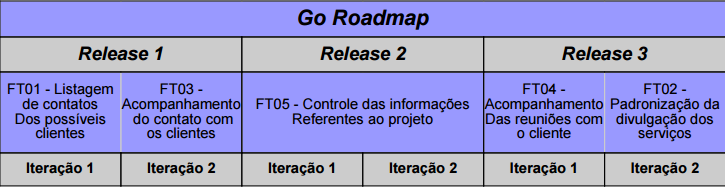
\includegraphics[scale=0.4]{figuras/roadmap.png}
\caption{\textit{Roadmap} do projeto}
\label{roadmap}
\end{figure}

\pagebreak

\section{Planejamento da Primeira \textit{Release}}

\subsection{Divisão das \textit{Features} em iterações}
O planejamento da \textit{Release} 1 foi feito considerando as necessidades do cliente e as restrições do time.
De acordo com o que foi definido no \textit{Roadmap}, será implementado na \textit{Release} 1 as \textit{Features}: FT-01 e FT-03. A partir disso, foi feita uma alocação das \textit{Features} em iterações que serão realizadas nesta \textit{Release}.

Para esta \textit{Release} foram definidas 4 iterações, mas dependendo do decorrer da execução da \textit{Release} pode haver a necessidade do planejamento de outras. 

Para a primeira e segunda iteração ficou decidido que serão implementadas as histórias derivadas da FT-01, pois, para o desenvolvimento das outras \textit{Features}, há a necessidade de informações que esta \textit{Feature} irá submeter.

Para a terceira e quarta iteração foi definido o desenvolvimento das histórias de usuário derivadas da FT-03. A FT-03 foi definida para depois da  FT-01, pois para o desenvolvimento dela são necessárias informações vindas FT-01, tais como o registro de um contato realizado com o cliente.

\begin{figure}[!htb]
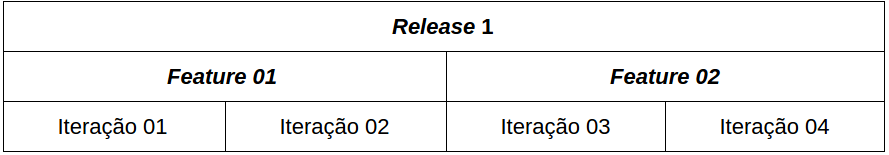
\includegraphics[scale=0.5]{figuras/planejamento_release.png}
\caption{Divisão das \textit{Features} em iterações}
\label{fig:backlog}
\end{figure}

\subsection{Critérios de aceitação das \textit{Features} da Release}
Também foram escritos os critérios de aceitação das \textit{features} pertencentes da primeira \textit{Release}.

      \textbf{FT-01 Listagem de contatos dos possíveis clientes}
      \begin{itemize}
       \item Deve ser acessado pelos membros equipe de marketing;
       \item As informações do cliente devem estar organizadas em duas divisões: básicas e detalhadas;
       \item Deve ser possível ter uma visualização completa e detalhada do cliente;
       \item Essas informações devem estar organizadas em formato de abas, cada uma em uma aba diferente.
      \end{itemize}
      
      \textbf{FT03 - Acompanhamento do contato com o cliente}
      \begin{itemize}
       \item Deve haver uma diferenciação entre os clientes contatados e os não contatados.
      \end{itemize}

